\documentclass{article}
\usepackage{tkz-euclide} % loads  TikZ and tkz-base
\begin{document}

\title{AI1110 Software Project Report}
\author{Name:Dikshant Khandelwal\\
        Roll Number:CS22BTECH11017}

\maketitle

\section{Introduction}
The Music Player project is a simple music player application built using the Pygame library in Python. It allows users to play and control the playback of audio files. The application provides basic functionalities such as playing the next or previous song, pausing and resuming the playback, and displaying the currently playing song.

\section{Implementation}
The project is implemented using the Pygame library, which provides functionality for graphics and audio in Python. The code is organized into classes and functions to handle different aspects of the music player.

\subsection{Dependencies}
The following dependencies are required to run the Music Player:
\begin{itemize}
\item Python 
\item Pygame library
\item NumPy library
\end{itemize}
Additional dependencies are:
\begin{itemize}
        \item sys Module
        \item os Module
\end{itemize}

\subsection{Code Structure}
The code is structured as follows:

\begin{itemize}
\item Importing necessary libraries and initializing Pygame.
\item Defining color constants using Pygame's Color class.
\item Creating the Pygame screen and initializing the mixer for audio playback.
\item Defining a Button class to represent the control buttons in the music player.
\item Setting up the initial song list and play stack.
\item Creating instances of the Button class for previous, next, and play buttons.
\item Setting up the main loop to handle events and update the screen.
\item Handling button clicks and updating the play stack accordingly.
\item Loading and playing the selected song using Pygame's mixer.
\end{itemize}

\section{Conclusion}
The Music Player project provides a basic music player application with features such as playing audio files, controlling playback, and displaying the currently playing song. It demonstrates the use of Pygame and its audio capabilities in Python programming.


\section{Images}
\begin{figure}[h!]
        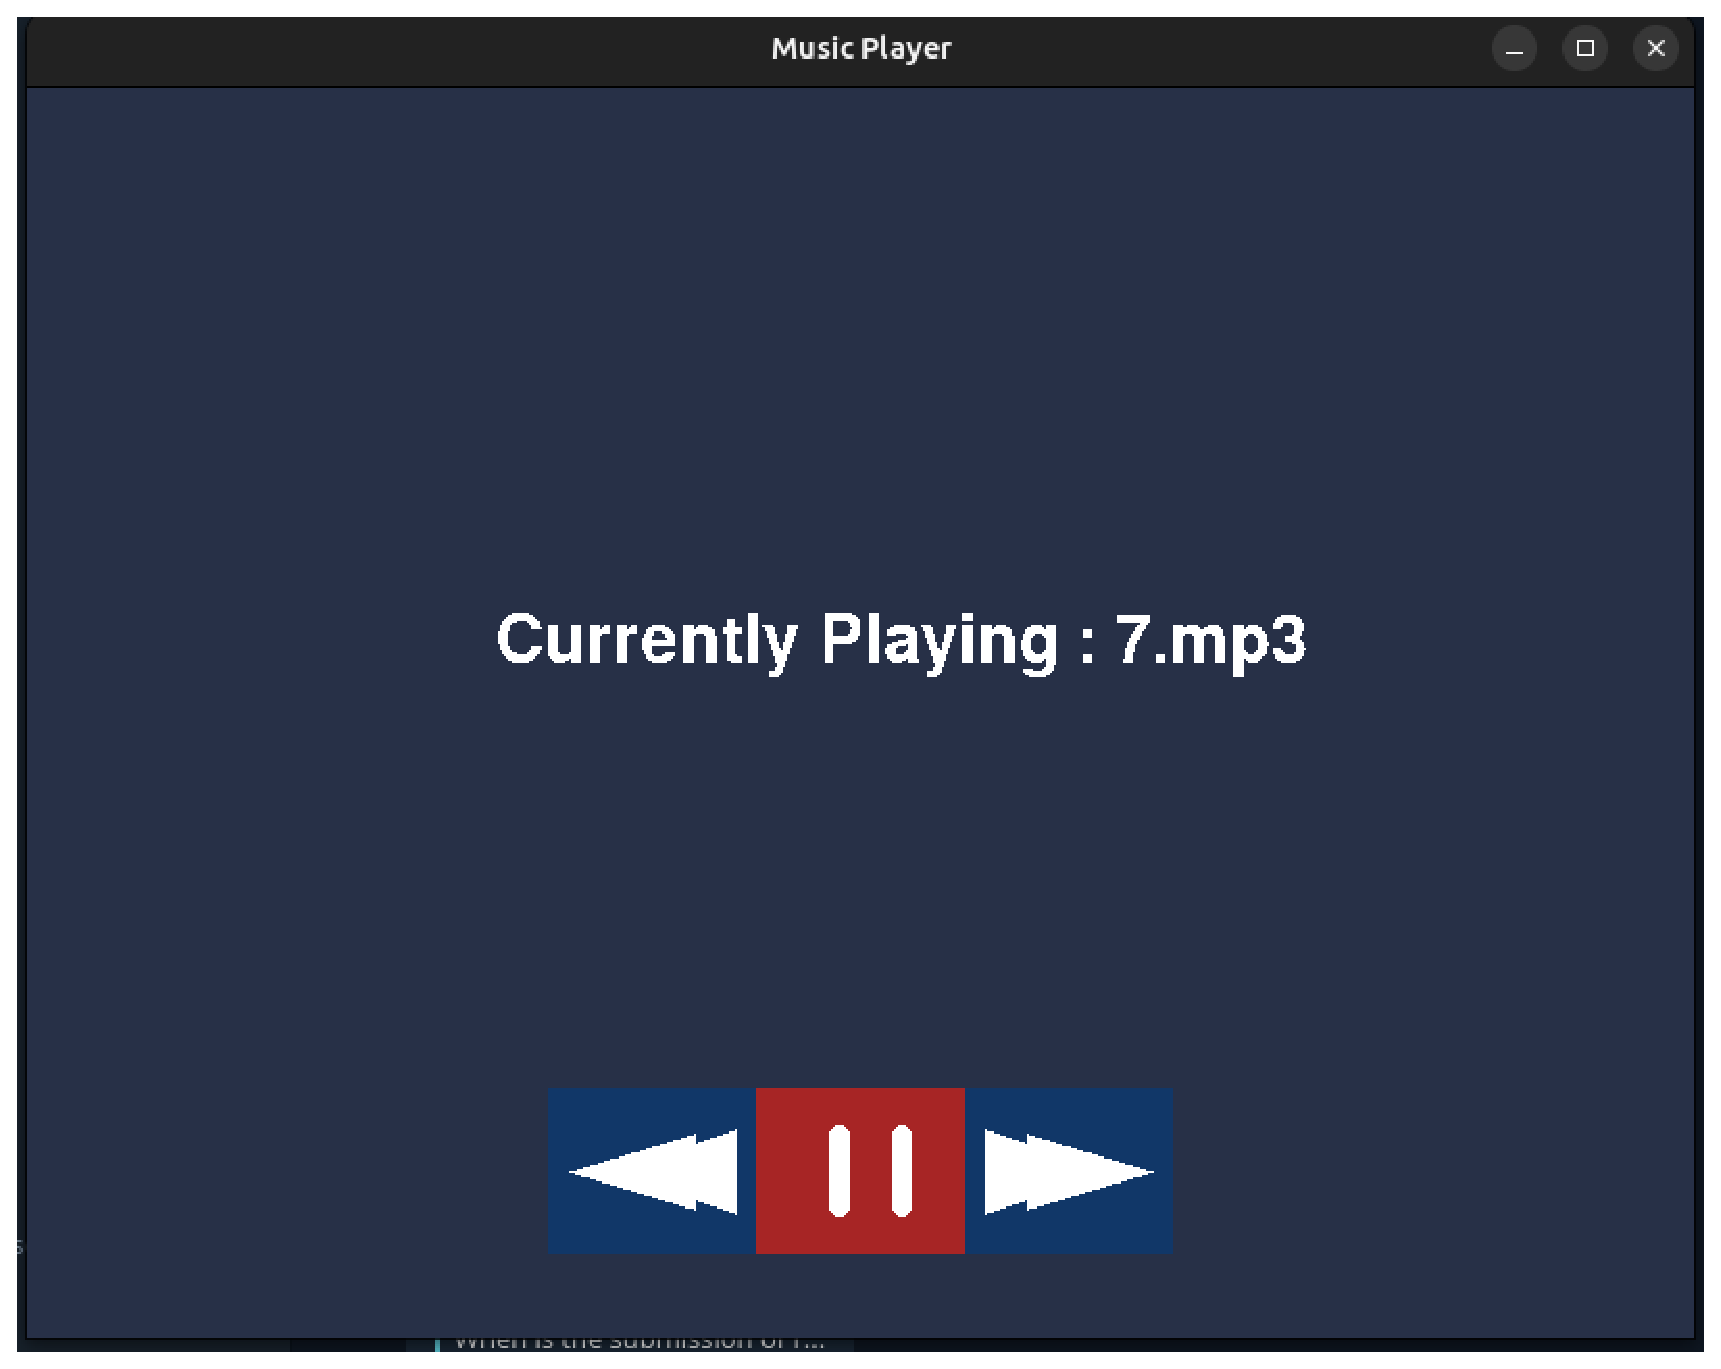
\includegraphics[scale = 0.25]{figs/img1}
        \caption{First Song(Paused)}
        \label{fig:1}
\end{figure}

\begin{figure}[h!]
        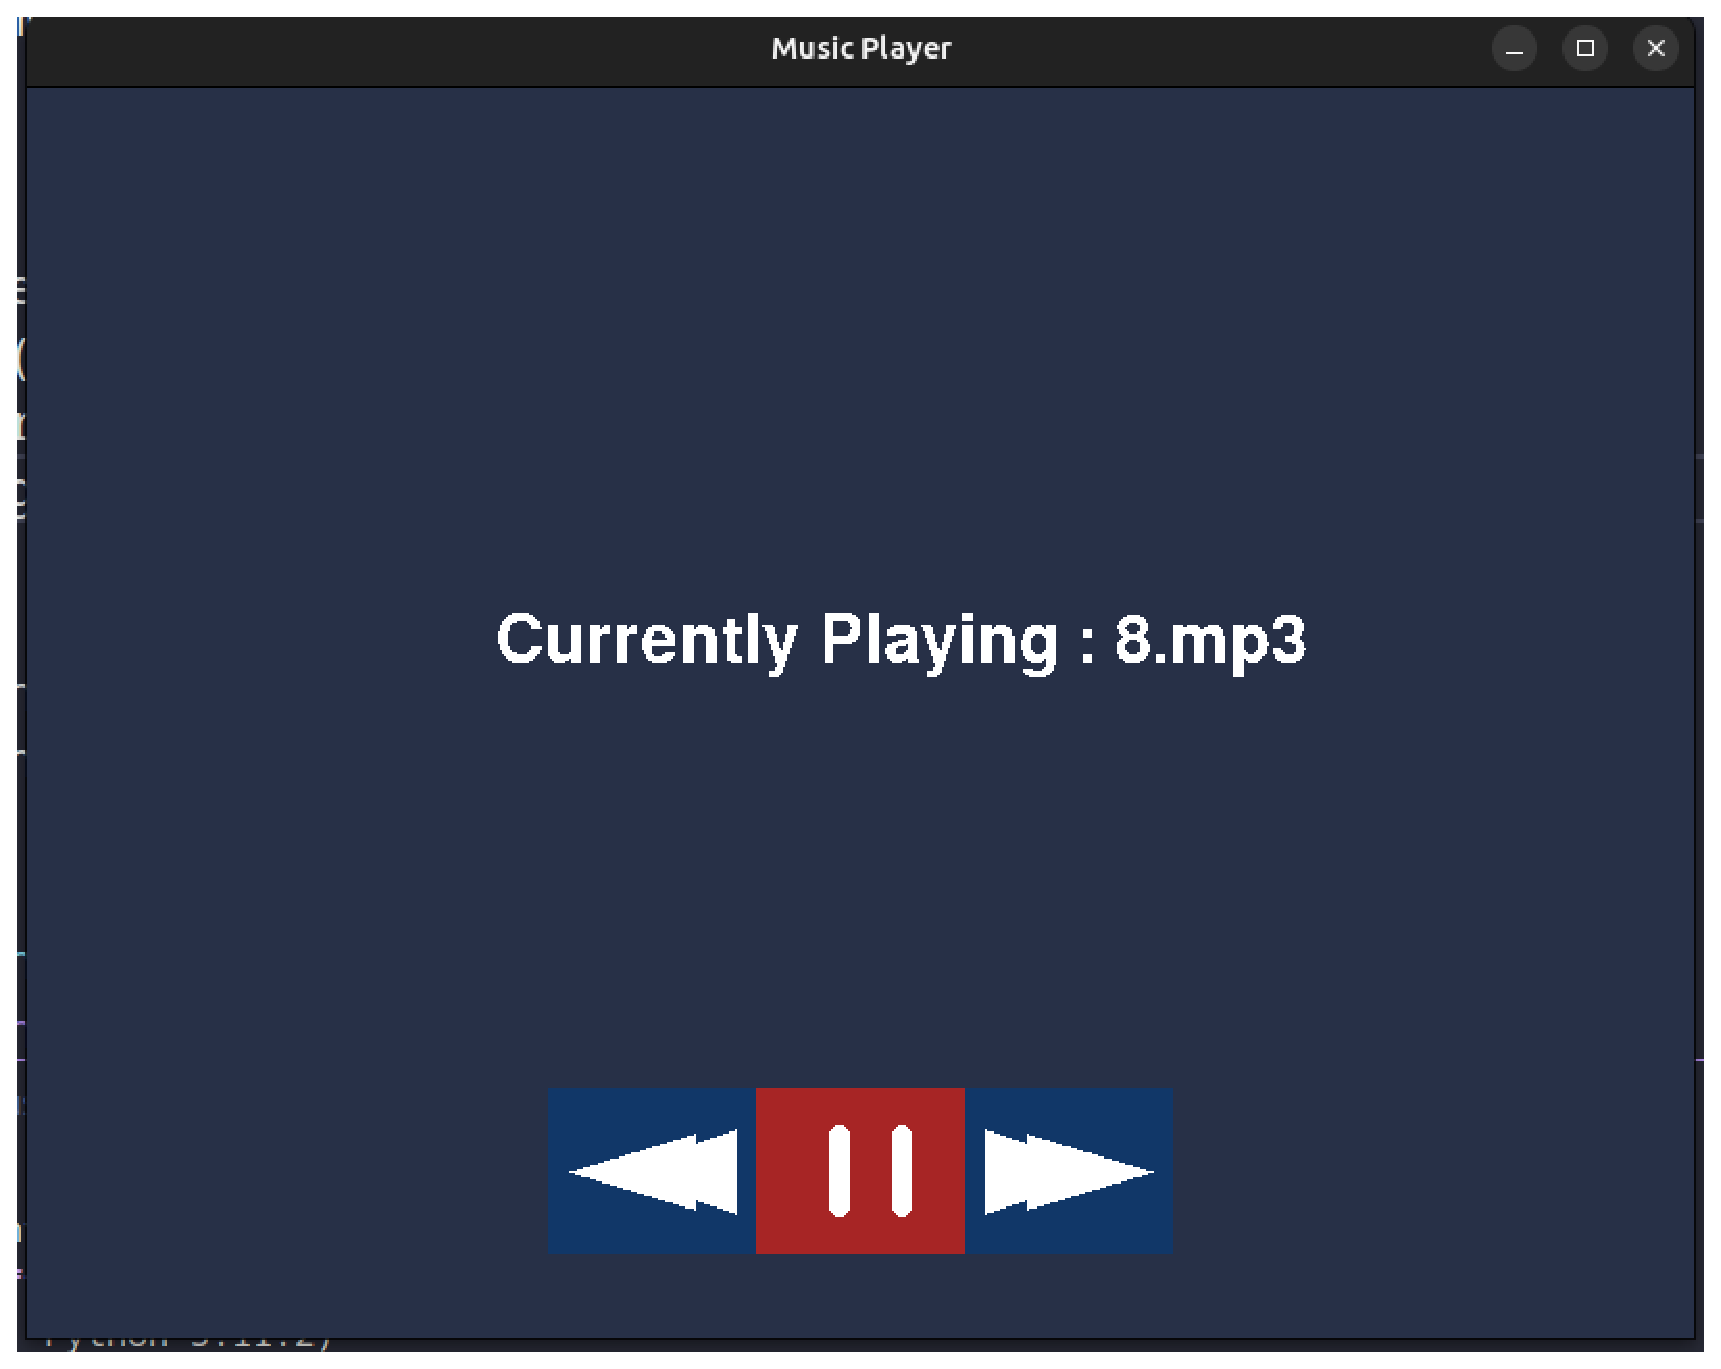
\includegraphics[scale = 0.25]{figs/img2}
        \caption{Second Song(Paused)}
        \label{fig:2}
\end{figure}

\begin{figure}[h!]
       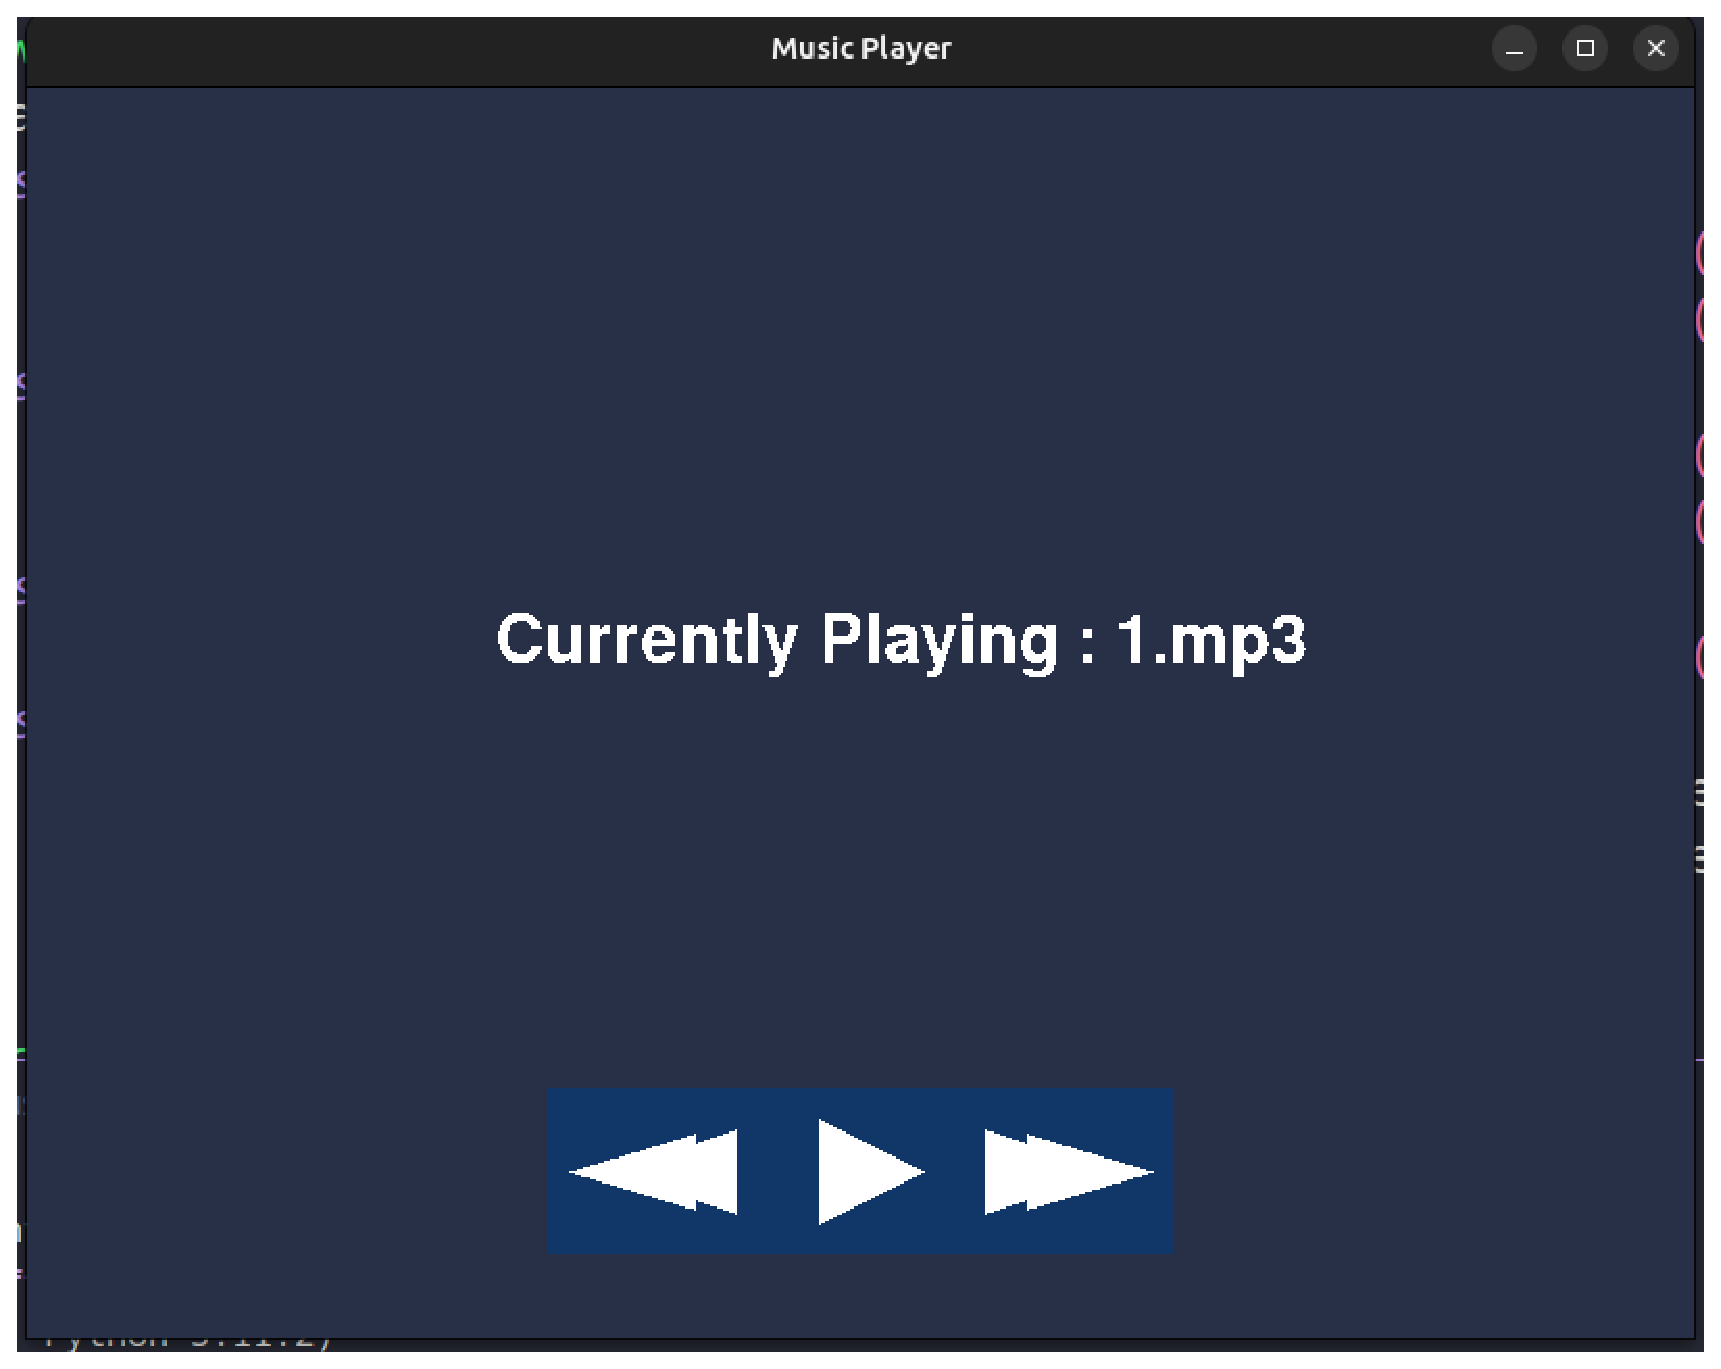
\includegraphics[scale = 0.25]{figs/img3}
        \caption{Third Song(Playing)}
        \label{fig:3}
\end{figure}

The code for the Music Player can be found at:
\textbf{https://github.com/DikshantK2004/Music-Player}
\end{document}